\documentclass[handout, 10pt]{beamer}
\usepackage[hangul]{kotex}
\usepackage[T1]{fontenc}

% other packages
\usepackage{natbib}
\usepackage{graphicx,float,pstricks,listings,stackengine,xcolor,calligra}
\usepackage{amsmath,amssymb,latexsym}
\usepackage{booktabs,longtable,multicol,multirow,lscape,rotating,subfig}
\usepackage{caption,subcaption}
    \newcommand{\source}[1]{\subcaption*{\raggedright 자료: {#1} } }
\usepackage{threeparttable} % Align column caption, table, and notes
\usepackage{adjustbox} % Shrink stuff
%\usepackage{showframe} % Useful for debugging

\author{오성재}
\title{기회불평등과 경제성장}
%\subtitle{}
\institute{한남대학교 탈메지이 교양학부}
\date{\today}
\usetheme{Darmstadt}
\usecolortheme{seahorse}
%\usepackage{warehouse/PekingU}

% defs
\def\cmd#1{\texttt{\color{red}\footnotesize $\backslash$#1}}
\def\env#1{\texttt{\color{blue}\footnotesize #1}}
\definecolor{deepblue}{rgb}{0,0,0.5}
\definecolor{deepred}{rgb}{0.6,0,0}
\definecolor{deepgreen}{rgb}{0,0.5,0}
\definecolor{halfgray}{gray}{0.55}

\lstset{
    basicstyle=\ttfamily\small,
    keywordstyle=\bfseries\color{deepblue},
    emphstyle=\ttfamily\color{deepred},    % Custom highlighting style
    stringstyle=\color{deepgreen},
    numbers=left,
    numberstyle=\small\color{halfgray},
    rulesepcolor=\color{red!20!green!20!blue!20},
    frame=shadowbox,
}


\begin{document}

\begin{frame}
    \titlepage
    %\begin{figure}[htpb]
        %\begin{center}
            %
\includegraphics[width=0.2\linewidth]{pic/PKU_logo.png}
        %\end{center}
    %\end{figure}
\end{frame}

%\AtBeginSection[]
%{
  %\begin{frame}
    %\frametitle{Table of Contents}
    %\tableofcontents[sectionstyle=show,subsectionstyle=show/shaded/hide,subsubsectionstyle=show/shaded/hide,currentsection]
  %\end{frame}
%}

\begin{frame}
    \frametitle{Table of Contents}
    \tableofcontents[sectionstyle=show,subsectionstyle=show/shaded/hide,subsubsectionstyle=show/shaded/hide]
\end{frame}

\section{문제제기}
\begin{frame}
    \begin{itemize}
        \item 불평등과 경제성장의 단기 관계에 대한 실증연구는 다양한 결과를 제시함.
    \end{itemize}
    \begin{figure}[htpb]
        \begin{center}
            \caption{경제성장, 불평등 그리고 빈곤의 관계}
            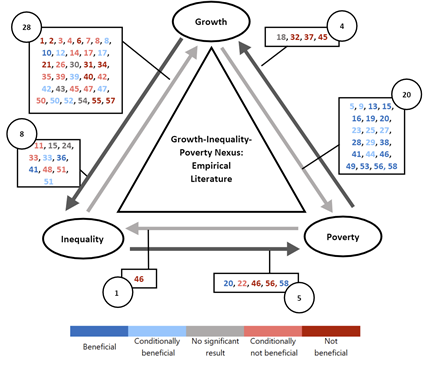
\includegraphics[scale=0.35]{pic/triangle_relations.png}
        \end{center}
    \end{figure}
\end{frame}

\section{불평등과 빈곤의 추세}
\begin{frame}[<+->]
\frametitle{불평등의 추세}
    \begin{itemize}
        \item 선진국에서 시장소득 불평등은 증가하였다. 반면, 신흥국과 개도국에서의 불평등은 일정한 모습이다.
    \end{itemize}
    \begin{figure}[htpb]
        \begin{center}
            \caption{국가집단별 불평등, 1980년대-2010년대}
            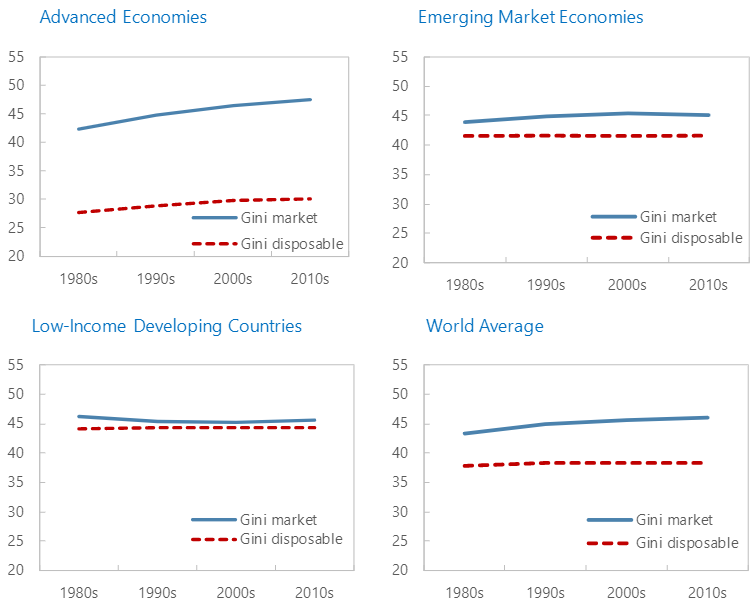
\includegraphics[scale=0.3]{pic/Inequality across Country Group.png}
        \end{center}
    \end{figure}
\end{frame}


\begin{frame}[<+->]
\frametitle{}
    \begin{table}[htbp]
        \begin{adjustbox}{width=\textwidth, totalheight=\textheight-2\baselineskip,keepaspectratio}
            \begin{threeparttable}
                \caption{1980년대와 2010년대의 빈곤, 불평등 비교}
                      \centering
        \begin{tabular}{lrrr|rrr}
        \toprule
        Country & 지니계수 (1980s) & 지니계수 (2010s) & 지니계수 변화 & 빈곤률 (1980s) & 빈곤률 (2010s) & 빈곤률 변화 \\
        \midrule
        Brazil & 60.9  & 55.2  & -5.8  & 37.5  & 8.6   & -28.9 \\
        Canada & 40.7  & 45.5  & 4.7   & 0.4   & 0.4   & 0 \\
        China & 30.2  & 41.4  & 11.2  & ... & 15.2  & ... \\
        France & 48.2  & 49    & 0.8   & 1.6   & 0.1   & -1.5 \\
        Germany & 42.5  & 51.9  & 9.4   & ... & 0.1   & ... \\
        India & 42.1  & 49    & 6.9   & 84.9  & 61.7  & -23.2 \\
        Indonesia & 39.6  & 42.6  & 3.1   & 91.1  & 33.9  & -57.2 \\
        Italy & 43.9  & 49.3  & 5.4   & 0.8   & 1.9   & 1.1 \\
        Japan & 37.8  & 45.6  & 7.8   & ... & 0.6   & ... \\
        Mexico & 46.8  & 47.2  & 0.4   & 19    & 10.2  & -8.8 \\
        Russia & 35.3  & 45.6  & 10.4  & ... & 0.5   & ... \\
        South Africa & 65.7  & 68.5  & 2.8   & ... & 36.4  & ... \\
        Turkey & 44.4  & 43.1  & -1.3  & 13.2  & 2.6   & -10.6 \\
        United Kingdom & 46.4  & 52.9  & 6.5   & 1.2   & 0.3   & -0.9 \\
        United States & 44.7  & 50.8  & 6.1   & 0.7   & 1.2   & 0.5 \\
        \midrule
        Country classification &       &       &       &       &       &  \\
        Advanced economies & 42.6  & 46.9  & 4.3   & 0.8   & 0.5   & -0.3 \\
        Emerging markets & 44.9  & 45.1  & 0.2   & 34.7  & 9     & -25.7 \\
        Low-income developing countries & 46.2  & 44.9  & -1.2  & 62.3  & 46.4  & -16 \\
        \midrule
        World average & 44.3  & 45.5  & 1.2   & 29.1  & 12.1  & -16.9 \\
        \bottomrule
        \end{tabular}%
            \end{threeparttable}
        \end{adjustbox}
    \end{table}
\end{frame}

\begin{frame}[<+->]
\frametitle{불평등지수의 다양성}
    \begin{itemize}
        \item 선진국 집단에서 불평등지수의 크기는 거의 같다. 반면 신흥국과 개도국 집단에서 불평등 지수는 다양하다.
    \end{itemize}
    \begin{figure}[htpb]
        \begin{center}
            \caption{국가집단별 불평등지수}
            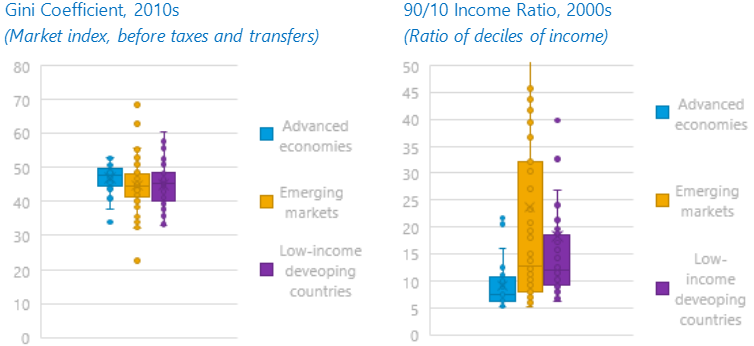
\includegraphics[scale=0.35]{pic/Indicators of Inequality across Country Groups.png}
        \end{center}
    \end{figure}
\end{frame}

\begin{frame}[<+->]
\frametitle{빈곤률 변화}
    \begin{itemize}
        \item 신흥국은 지난 40년간 빈곤률이 크게 하락하였다.
    \end{itemize}
    \begin{figure}[htpb]
        \begin{center}
            \caption{국가집단별 빈곤률}
            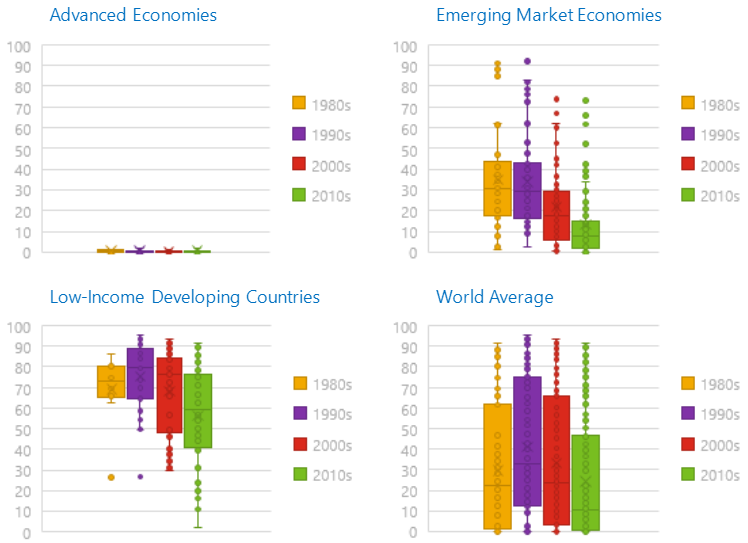
\includegraphics[scale=0.35]{pic/Poverty across Country Groups.png}
        \end{center}
    \end{figure}
\end{frame}

\begin{frame}[<+->]
\frametitle{경제성장률 변화}
    \begin{itemize}
        \item 선진국의 경제성장률은 하락하는 추세이다. 반면 신흥국과 개도국의 경제성장률은 상승하고 있다.
    \end{itemize}
    \begin{figure}[htpb]
        \begin{center}
            \caption{국가집단별 경제성장률 추이}
            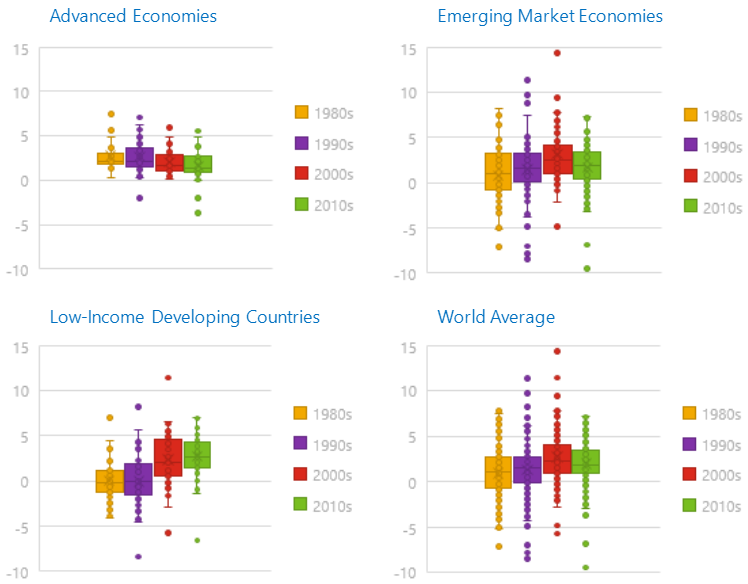
\includegraphics[scale=0.35]{pic/Average Growth in GDP per capita across Country Groups.png}
        \end{center}
    \end{figure}
\end{frame}


\begin{frame}[<+->]
\frametitle{}
    \begin{itemize}
        \item 1인당 GDP 성장은 빈곤층 소득의 상승과 강한 상관관계를 가진다.
    \end{itemize}
    \begin{figure}%
        \centering
        \caption{최하위층 소득과 1인당 GDP 그리고 성장률}%
        \subfloat{{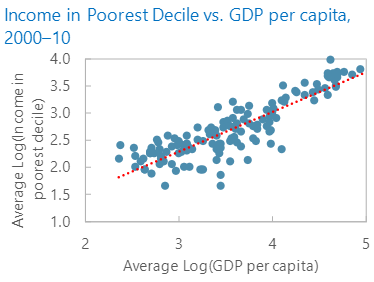
\includegraphics[width=.45\textwidth]{pic/Income in Poorest Decile vs. GDP per capita.png}}}%
        \qquad
        \subfloat{{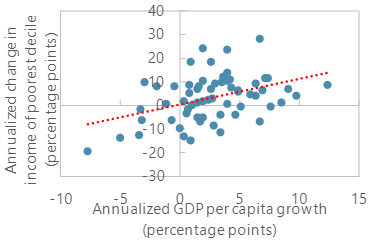
\includegraphics[width=.45\textwidth]{pic/Change in Income of Poorest Decile and GDP per capita Growth.png} }}%
    \end{figure}
\end{frame}

\begin{frame}[<+->]
\frametitle{}
    \begin{itemize}
        \item 1인당 GDP 성장과 전반적인 불평등과의 관계는 불분명 하다.
    \end{itemize}
    \begin{figure}%
        \centering
        \caption{시장소득 지니계수와 1인당 GDP 그리고 성장률}%
        \subfloat{{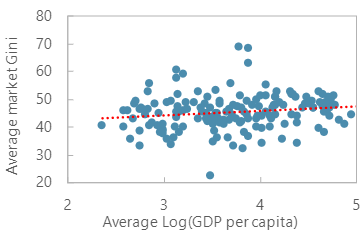
\includegraphics[width=.45\textwidth]{pic/Market Gini and GDP per capita.png}}}%
        \qquad
        \subfloat{{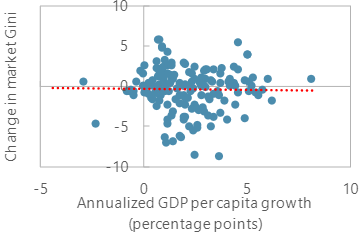
\includegraphics[width=.45\textwidth]{pic/Change in Market Gini and GDP per capita Growth.png} }}%
    \end{figure}
\end{frame}

\section{빈곤 및 소득이 경제성장에 미치는 영향}

\begin{frame}[<+->]
\frametitle{빈곤이 경제성장에 미치는 영향}
    \begin{itemize}
        \item 빈곤률이 높았던 국가는 낮은 경제성장률을 보임. 
    \end{itemize}
    \begin{figure}[htpb]
        \begin{center}
            \caption{빈곤률(1960년)과 경제성장률(1960-2010)}
            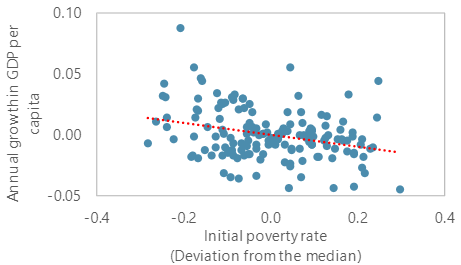
\includegraphics[scale=0.5]{pic/Growth in GDP per capita vs Initial Poverty.png}
        \end{center}
    \end{figure}
\end{frame}

\begin{frame}[<+->]
\frametitle{불평등과 경제성장 간의 관계}
    \begin{itemize}
        \item 불평등이 낮은 수준이었던 국가가 경제성장룰도 높음.
    \end{itemize}
    \begin{figure}[htpb]
        \begin{center}
            \caption{초기불평등과 경제성장률}
            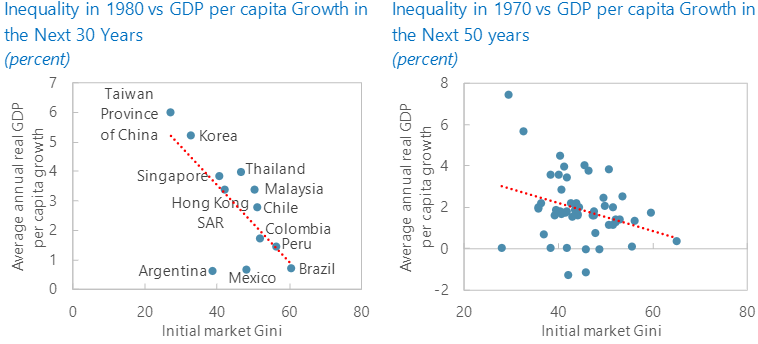
\includegraphics[scale=0.5]{pic/Growth in GDP per capita vs Initial Inequality.png}
        \end{center}
    \end{figure}
\end{frame}

\begin{frame}[<+->]
\frametitle{빈곤의 함정(poverty trap)과 인적자본}
    \begin{itemize}
        \item 빈곤률이 높은 국가에서 보건지출이 낮다.
    \end{itemize}
    \begin{figure}%
        \centering
        \caption{빈곤과 보건수준의 관계}%
        \subfloat{{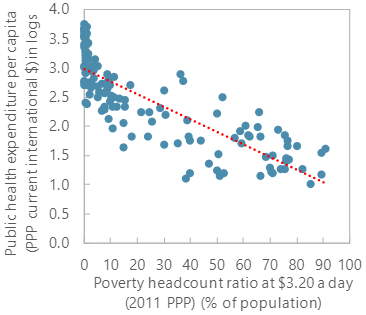
\includegraphics[width=.45\textwidth]{pic/Poverty Rate vs Expenditure on Public Health.png}}}%
        \qquad
        \subfloat{{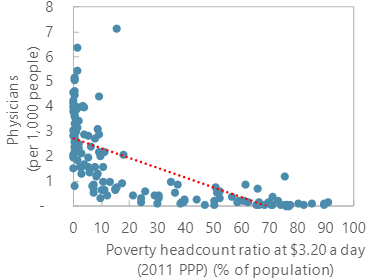
\includegraphics[width=.45\textwidth]{pic/Poverty Rate vs Coverage of Doctors.png} }}%
    \end{figure}
\end{frame}

\begin{frame}[<+->]
\frametitle{빈곤의 함정(poverty trap)과 인적자본}
    \begin{itemize}
        \item 빈곤률이 높은 국가에서 교육지출도 낮다.
    \end{itemize}
    \begin{figure}%
        \centering
        \caption{빈곤과 교육수준의 관계}%
        \subfloat{{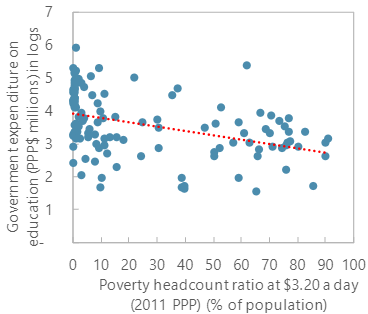
\includegraphics[width=.45\textwidth]{pic/Poverty Rate vs Expenditure on Public Education.png}}}%
        \qquad
        \subfloat{{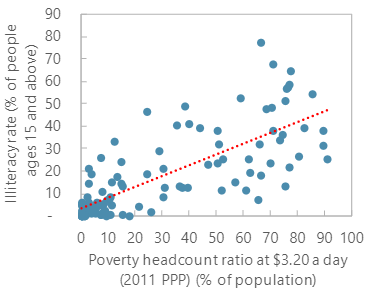
\includegraphics[width=.45\textwidth]{pic/Poverty Rate vs Illiteracy Rate.png} }}%
    \end{figure}
\end{frame}

\section{선행연구}

\subsection{불평등과 경제성장}
\begin{frame}{한 경제의 불평등이 경제성장에 미치는 효과}
    \begin{itemize}
        \item 이론적 연구
        \begin{itemize}
            \item 물적 자본.
            \item 인적 자본(\cite{gnz93}).
            \item 소득재분배(\cite{anr94}; \cite{pnt94}).
            \item 정치 불안정 등등.
        \end{itemize}
        \item 실증적 연구
        \begin{itemize}
            \item 횡단면 자료.
            \item 국가별 패널자료.
            \item 국가별 패널자료 $+$ 기타 고려사항.
        \end{itemize}
    \end{itemize}
\end{frame}

\begin{frame}{실증연구의 동향}
    \begin{itemize}
        \item 횡단면 자료: \cite{barro91}, \cite{anr94}, \cite{pnt94}
        \begin{itemize}
            \item 불평등은 경제성장에 부의 영향
        \end{itemize}
        \item 국가별 패널자료: \cite{lnz98}, \cite{barro20}, \cite{forbes00}, \cite{bnd03}
        \begin{itemize}
            \item 효과의 방향이 불확실, 부/영/정의 영향
        \end{itemize}
        \item 국가별 패널자료 + 국가별 이질성 및 세부 구성요인:
        \begin{itemize}
            \item \cite{voit05, voit11}: 중상위 불평등, 중하위 불평등
            \item \cite{cc10}: 중/저소득 vs. 고소득 국가 집단
            \item \cite{hetl14}: 단기 vs. 장기
        \end{itemize}
    \end{itemize}
\end{frame}


\subsection{기회불평등}
\begin{frame}{기회불평등과 경제성장}
    \begin{itemize}
        \item \cite{mnr13} : 미국내 주를 대상으로 연구를 진행하여 기회불평등이 경제성장에 부정적인 반면 잔여 불평등은 긍정적임을 보임.
        \begin{itemize}
            \item 미국의 50개 주가 분석대상, 1970-1990년대 말.
            \item 사람들의 자유로운 이동이 가능한 경우 기회불평등의 효과 추정치 편의.
        \end{itemize}
        \item \cite{fetl18} : 기회불평등과 경제성장의 관계에 대하여 연구를 진행. 총불평등과 기회불평등이 경제성장과 부의 관계를 가짐을 확인.
        \begin{itemize}
            \item 전 세계 42개국의 가구조사 및 건강조사 미시자료 이용, 1985-2005년.
            \item 경제적 기회의 핵심변수인 부모의 경제력 변수(부모의 학력, 소득, 재산 등)가 부재한 상태 에서 기회불평등도 측정.
        \end{itemize}
    \end{itemize}
\end{frame}

\begin{frame}{기회불평등과 경제성장}
    \begin{itemize}
        \item \cite{ane20} : 기회불평등과 소득불평등의 교차항을 통해 기회불평등한 국가에서 소득의 불평등이 경제성장과 부의 관계를 가짐을 보임.
        \begin{itemize}
            \item 기회불평등을 세대간 소득$\cdot$교육탄력성으로 측정.
            \item 성취에 대한 기회와 노력의 기여에 대한 구분이 없음.
        \end{itemize}
        \item \cite{kno17} : 교육의 불평등을 기회의 불평등과 잔여 불평등으로 분해. OECD 국가들의 경우 기회의 불평등은 경제성장에 부정적 영향을 주고 잔여 불평등은 경제성장에 긍정적 영향을 미침.
        \begin{itemize}
            \item 국제교육평가자료인 TIMSS를 사용.
            \item 기회불평등의 최소한으로 측정하는 불평등지수 사용.
        \end{itemize}
    \end{itemize}
\end{frame}

\section{연구방법}
\subsection{기회불평등지수}
\begin{frame}{기호}
    \begin{itemize}
        \item  $i$ : 개인, $(i \in \{1,\ldots,N \} )$.
        \item 환경변수 $C_{ic}$ : 개인 $i$의 성취에 영향을 주면서 그 개인이 스스로의 의지로 선택할 수 없는 요인.(부모의 소득, 학력, 인종, 성별 등등.).
        \item 환경 $C_i$ : 개인 $i$가 속한 환경변수$C_{ci}$ 들의 c-터플(c-turple) $C_i = (C_{1i}, \ldots , C_{ci})$. 
        \item 환경유형 $T= \{1, \ldots , t \}$, $t= ||C_1|| \times \cdots \times ||C_c||$ : 가능한 모든 환경의 지표(index).
    \end{itemize}
\end{frame}

\begin{frame}{성취, 환경 그리고 노력}
    \begin{itemize}
        \item 개인 $i$의 성취인 성적점수를 $y_i$, 그가 속한 환경을 $C_i$, 노력을 $e_i$라고 표시하자.
        \item 기회불평등의 관점에서 성취는 개인이 속한 환경 및 환경과 무관한 개인의 노력의 결과라고 정의한다.
        \item 개인 $i$ 성취 $y_i$는 환경 $C_i$ 및 노력 $e_i$에 대하여 다음의 선형함수관계를 가진다고 가정한다.
        \begin{equation}
            \label{eq:ols}
             y_{i} =\beta _0 +  \beta _1 C_{1i} + \cdots + \beta _c C_{ci} + \epsilon _i
        \end{equation}
    \end{itemize}
\end{frame}

\begin{frame}{\cite{fng11}}
    \begin{itemize}
        \item 성취의 불평등을 기회의 불평등과 노력의 불평등으로 분해하기 위해 가산적 분해가능성(additively decomposibility)이 있는 타일-0(Theil-0) 지수를 이용한다.
        \begin{equation}
            \label{eq:theil0}
            T(Y)=\frac{1}{N} \sum_{i=1}^{N} \ln \left(\frac{\bar{y}}{y_{i}}\right)
        \end{equation} 
        \item \cite{fng11}는 식 (\ref{eq:ols})을 식 (\ref{eq:theil0})에 대입하는 방법으로 기회불평등과 잔여불평등을 구분한다.
    \end{itemize}
    \begin{equation}
        \label{eq:theil0-decompose}
        T(Y)=T(C ' \cdot \beta) + T(\epsilon)
    \end{equation}
\end{frame}

\begin{frame}{순수한 노력}
    \begin{itemize}
        \item \cite{betl12}는 \cite{Roemer98}의 순수한 노력(pure effort) 개념을 도입하여 식 (\ref{eq:ols})에서 오차항에 존재하는 환경의 영향을 받는 성취를 찾는다.
        \item 오차항이 환경의 영향을 받는다면 조건부 분산 $\sigma ^2 _c = Var[\epsilon |C_c]$이 환경별로 상이할 것이다.
        \item 잔차의 총분산이 $\sigma ^2 =  \sum _c f_c \sigma ^2 _c$인 점을 이용해 오차항의 이분산성을 해소할 수 있다.
    \end{itemize}
\end{frame}

\begin{frame}{\cite{betl12}}
    \begin{itemize}
        \item  $k = ( 1 / \sum _c f _c \sigma ^2 _c ) ^{-1/2}$라고 한다면, 식 (\ref{eq:ols})을 아래와 같이 바꿀 수 있다. 
        \begin{equation}
            \label{eq:bjork}
            \begin{aligned} Y_{i} &= \beta _0 +  \beta _1 C_{1i} + \cdots + \beta _c C_{ci} + \epsilon_{i} \\ &= \beta _0 +  \beta _1 C_{1i} + \cdots + \beta _c C_{ci} +\epsilon_{i}-\underbrace{\epsilon_{i} / k \sigma_{c}}_{u_{i}}+\underbrace{\epsilon_{i} / k \sigma_{c}}_{u_{i}} \\ &= \beta _0 +  \beta _1 C_{1i} + \cdots + \beta _c C_{ci} +\widetilde{\epsilon}_{i}+u_{i}, \end{aligned}
        \end{equation}
        \item 식 (\ref{eq:theil0-decompose})은 아래와 같이 바꿀 수 있다.. 
        \begin{equation}
            \label{eq:theil0-bjork}
            T(Y)=T(C' \cdot \beta +\widetilde{\epsilon}) + T ( u )
        \end{equation}
        \item 위 식의 우변 첫번째 항은 기회의 불평등을 나타내고 두번째 항은 노력의 불평등이다.
    \end{itemize}
\end{frame}

\subsection{회귀분석모형}
\begin{frame}{회귀분석모형}
   \begin{itemize}
       \item  본 연구에서 우리는 성장 회귀분석(growth regression)에서 일반적으로 사용하는 다음의 실증모형을 추정한다.
       \item 회귀분석은 선형회귀분석(OLS), 패널 고정효과(fixed effect) 모형, 시스템 GMM(\cite{bnb98}) 방법을 적용함으로써 주요 계수들을 추정한다.
       \begin{equation}
            \begin{aligned}
            \ln \left(Y_{i, t^{\prime}}\right)-\ln \left(Y_{i, t}\right)=& \delta_{1} I O P_{i, t}+\delta_{2} I O E_{i, t}+\beta_{1} \ln \left(Y_{i, t}\right) \\
            &+X_{i, t} \beta_{2} +\alpha_{i}+\tau_{t^{\prime}}+u_{i, t^{\prime}}
            \end{aligned}
            \label{eq:regbase}
       \end{equation} 
   \end{itemize} 
\end{frame}
 
\begin{frame}{회귀분석모형의 기호}
   \begin{itemize}
        \item $i$ : 국가, $t$ : 교육기회불평등의 측정연도
        \item $t'$ : TIMSS의 경우 $t'=t+4$, PISA의 경우  $t'=t+3$
        \item $Y_{i,t}$ : 국가 $i$의 연도 $t$현재 1인당 GDP
        \item $IOP_{i,t}$ : 기회불평등 지수, $IOE_{i,t}$ : 노력 불평등의 지수
        \item $X_{i,t}$ : 국가 $i$의 $t$연도 현재 특성변수들(인구 수 및 투자재의 가격)의 벡터 
        \item $\alpha _i$ : 국가 고정효과, $\tau _{t'}$ : 연도 고정효과
   \end{itemize} 
\end{frame}

\section{자료소개}
\begin{frame}{TIMSS}
    \begin{itemize}
        \item TIMSS (Trends in International Mathematics and Science Study)
        \begin{itemize}
            \item 1995, 1999, 2003, 2007, 2011, 2015, 2019년도 조사
            \item 수학/과학 학업(curriculum)성취도 검사
            \item 4학년과 8학년 학생들을 대상으로 시행.
        \end{itemize}
    \end{itemize}
\end{frame}

\begin{frame}{PISA}
    \begin{itemize}
         \item PISA (Programme for International Student Assessment)
        \begin{itemize}
            \item 2000, 2003, 2006, 2009 , 2012, 2015, 2018년도 조사
            \item 읽기/수학/과학 문해력(literacy) 검사
            \item 만 15세 대상으로 시행.
        \end{itemize}
    \end{itemize}
\end{frame}

\begin{frame}{추가 자료설명}
    \begin{itemize}
        \item Penn World Table로부터 국가별 1인당 GDP 및 인구, 투자재의 가격 등 거시 통제변수 구축.
        \item 공통사항
        \begin{itemize}
            \item 학생의 개인/가정/교사/학교 정보 조사.
            \item 각 조사마다 34-77개 국가 참가, 총 98개국의 성적 자료.
            \item 전세계 참여학생의 수학성적을 평균 500 분산 100점으로 정규화.
        \end{itemize}
    \end{itemize}
\end{frame}

\begin{frame}{환경변수}
    \begin{itemize}
    \item 부친 및 모친모의 학력 :
    \begin{itemize}
        \item ISCED Lv에 따라 분류(1-7)를 단순 합산하여 2-14의 값을 취함.
    \end{itemize}
    \item 장서수 :
    \begin{itemize}
        \item (1) 10권 미만 - (5) 200권 초과
    \end{itemize}
    \item 가정내 소유물
    \begin{itemize}
        \item 책상, 학생방, 컴퓨터, 인터넷 등 4개 항목을 더미로 조사하여 합산(0-4)
    \end{itemize}
    \item 최대 325개(=13$\times$5$\times$5)의 독립적인 환경 조합을 구성하여 기회불평등의 비중 계산
    \end{itemize}
\end{frame}

\begin{frame}{PISA와 TIMSS의 자료 차이: 응답률}
    \begin{figure}[htpb]
        \begin{center}
            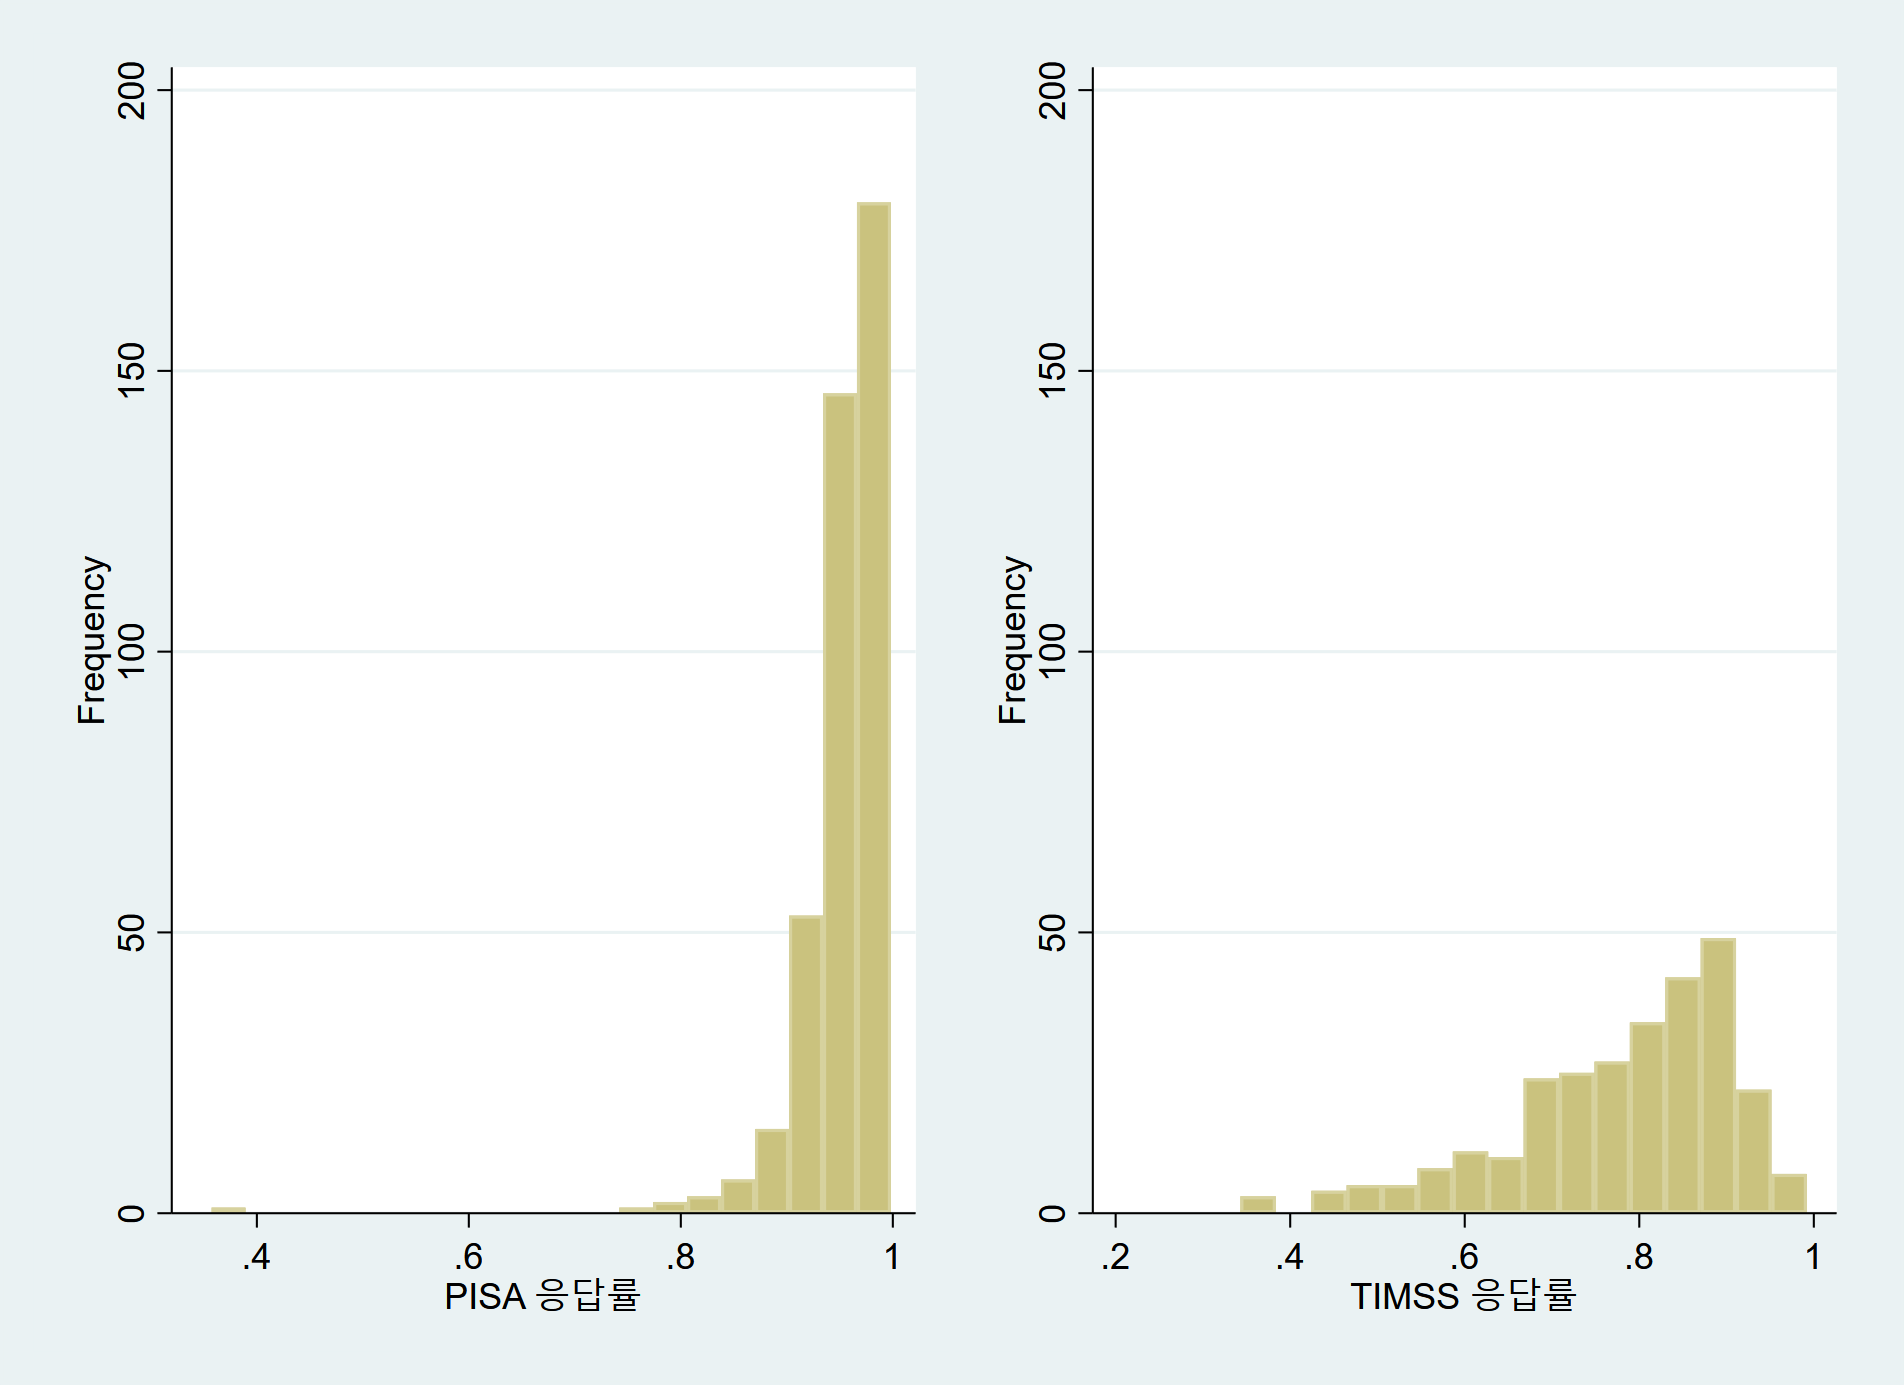
\includegraphics[scale=0.08]{pic/pnt_response.png}
            \caption{PISA와 TIMSS 환경변수 응답률}
        \end{center}
    \end{figure}
    \begin{itemize}
        \item TIMSS의 경우 학생이 자신의 가정환경을 응답하므로 환경변수를 활용하는 본 연구는 해당자료 사용에서 응답률의 문제를 안고 있음.
    \end{itemize}
\end{frame}

\begin{frame}{PISA와 TIMSS의 자료 차이: 학업성취도 vs. 문해력}
    \begin{figure}[htpb]
        \begin{center}
            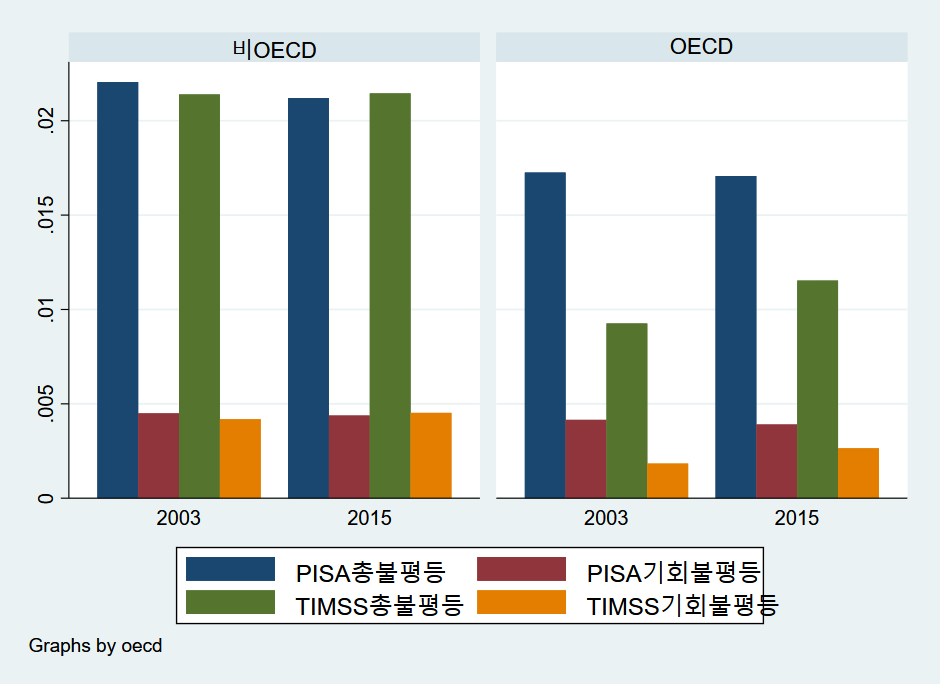
\includegraphics[scale=0.1]{pic/bar_pntcompare.png}
            \caption{PISA와 TIMSS 불평등 비교}
        \end{center}
    \end{figure}
    \begin{itemize}
        \item 국가별 성적의 평균을 중심으로 살펴볼때 학업성취도와 문해력은 매우 밀접한 관계를 보임.
        \item 국가별 성적의 분포를 중심으로 살펴보면 교육제도가 잘 갖춰진 국가일수록 두 교육성취는 차이를 보임. 
    \end{itemize}
\end{frame}

\section{주요결과}
\subsection{교육불평등지수}
\begin{frame}
    \begin{figure}[htpb]
        \begin{center}
            \includegraphics<1| handout:1>[scale=0.15]{pic/map_bjtpisa_mean.png}
            \includegraphics<2| handout:0>[scale=0.15]{pic/map_bjtpisa_2000.png}
            \includegraphics<3| handout:0>[scale=0.15]{pic/map_bjtpisa_2003.png}
            \includegraphics<4| handout:0>[scale=0.15]{pic/map_bjtpisa_2006.png}
            \includegraphics<5| handout:0>[scale=0.15]{pic/map_bjtpisa_2009.png}
            \includegraphics<6| handout:0>[scale=0.15]{pic/map_bjtpisa_2012.png}
            \includegraphics<7| handout:0>[scale=0.15]{pic/map_bjtpisa_2015.png}
            \includegraphics<8| handout:0>[scale=0.15]{pic/map_bjtpisa_2018.png}
            \caption{PISA 총불평등}
        \end{center}
    \end{figure}
\end{frame}

\begin{frame}
    \begin{figure}[htpb]
        \begin{center}
            \includegraphics<1| handout:1>[scale=0.15]{pic/map_bjrpisa_mean.png}
            \includegraphics<2| handout:0>[scale=0.15]{pic/map_bjrpisa_2000.png}
            \includegraphics<3| handout:0>[scale=0.15]{pic/map_bjrpisa_2003.png}
            \includegraphics<4| handout:0>[scale=0.15]{pic/map_bjrpisa_2006.png}
            \includegraphics<5| handout:0>[scale=0.15]{pic/map_bjrpisa_2009.png}
            \includegraphics<6| handout:0>[scale=0.15]{pic/map_bjrpisa_2012.png}
            \includegraphics<7| handout:0>[scale=0.15]{pic/map_bjrpisa_2015.png}
            \includegraphics<8| handout:0>[scale=0.15]{pic/map_bjrpisa_2018.png}
            \caption{PISA 기회불평등의 비중}
        \end{center}
    \end{figure}
\end{frame}

\begin{frame}
    \begin{figure}[htpb]
        \begin{center}
            \includegraphics<1| handout:1>[scale=0.15]{pic/map_bjttimss_mean.png}
            \includegraphics<2| handout:0>[scale=0.15]{pic/map_bjttimss_1995.png}
            \includegraphics<3| handout:0>[scale=0.15]{pic/map_bjttimss_1999.png}
            \includegraphics<4| handout:0>[scale=0.15]{pic/map_bjttimss_2003.png}
            \includegraphics<5| handout:0>[scale=0.15]{pic/map_bjttimss_2007.png}
            \includegraphics<6| handout:0>[scale=0.15]{pic/map_bjttimss_2011.png}
            \includegraphics<7| handout:0>[scale=0.15]{pic/map_bjttimss_2015.png}
            \includegraphics<8| handout:0>[scale=0.15]{pic/map_bjttimss_2019.png}
            \caption{TIMSS 총불평등}
        \end{center}
    \end{figure}
\end{frame}

\begin{frame}
    \begin{figure}[htpb]
        \begin{center}
            \includegraphics<1| handout:1>[scale=0.15]{pic/map_bjrtimss_mean.png}
            \includegraphics<2| handout:0>[scale=0.15]{pic/map_bjrtimss_1995.png}
            \includegraphics<3| handout:0>[scale=0.15]{pic/map_bjrtimss_1999.png}
            \includegraphics<4| handout:0>[scale=0.15]{pic/map_bjrtimss_2003.png}
            \includegraphics<5| handout:0>[scale=0.15]{pic/map_bjrtimss_2007.png}
            \includegraphics<6| handout:0>[scale=0.15]{pic/map_bjrtimss_2011.png}
            \includegraphics<7| handout:0>[scale=0.15]{pic/map_bjrtimss_2015.png}
            \includegraphics<8| handout:0>[scale=0.15]{pic/map_bjrtimss_2019.png}
            \caption{TIMSS 기회불평등의 비중}
        \end{center}
    \end{figure}
\end{frame}

\subsection{성장회귀분석}
\begin{frame}
    \begin{table}[htbp]
        \begin{adjustbox}{width=\textwidth, totalheight=\textheight-2\baselineskip,keepaspectratio}
            \begin{threeparttable}
                \centering
\def\sym#1{\ifmmode^{#1}\else\(^{#1}\)\fi}
\caption{PISA 총불평등\label{tab:pisasimp}}
\begin{tabular}{l*{6}{c}}
\toprule
                    &\multicolumn{1}{c}{(1)}&\multicolumn{1}{c}{(2)}&\multicolumn{1}{c}{(3)}&\multicolumn{1}{c}{(4)}&\multicolumn{1}{c}{(5)}&\multicolumn{1}{c}{(6)}\\ &\multicolumn{1}{c}{OLS}&\multicolumn{1}{c}{FE}&\multicolumn{1}{c}{Sys. GMM}&\multicolumn{1}{c}{OLS}&\multicolumn{1}{c}{FE}&\multicolumn{1}{c}{Sys. GMM}\\
\midrule
ln1인당GDP        &       0.931\sym{***}&       0.601\sym{***}&       0.817\sym{***}&       0.932\sym{***}&       0.602\sym{***}&       0.797\sym{***}\\
                    &     [58.96]         &     [14.25]         &     [12.91]         &     [54.78]         &     [14.31]         &     [11.49]         \\
\addlinespace
총불평등          &      -3.248\sym{***}&      -4.625\sym{***}&      -2.332         &                     &                     &                     \\
                    &     [-2.99]         &     [-3.27]         &     [-0.58]         &                     &                     &                     \\
\addlinespace
OECD$ \times$ 총불평등&                     &                     &                     &      -3.562\sym{***}&      -2.107         &       0.737         \\
                    &                     &                     &                     &     [-2.70]         &     [-0.95]         &      [0.12]         \\
\addlinespace
OECD$ \times$ 총불평등&                     &                     &                     &      -3.268\sym{***}&      -4.875\sym{***}&      -3.968         \\
                    &                     &                     &                     &     [-3.00]         &     [-3.43]         &     [-1.08]         \\
\addlinespace
투자재가격        &     -0.0552         &      -0.139\sym{**} &      0.0206         &     -0.0509         &      -0.148\sym{**} &     -0.0433         \\
                    &     [-1.21]         &     [-2.32]         &      [0.13]         &     [-1.17]         &     [-2.46]         &     [-0.40]         \\
\addlinespace
ln인구            &    -0.00777\sym{**} &      -0.200\sym{**} &      -0.184\sym{**} &    -0.00737\sym{**} &      -0.209\sym{**} &      -0.186\sym{**} \\
                    &     [-2.36]         &     [-2.23]         &     [-2.03]         &     [-2.18]         &     [-2.32]         &     [-2.15]         \\
\addlinespace
Constant            &       0.968\sym{***}&       4.886\sym{***}&       2.495\sym{***}&       0.957\sym{***}&       4.874\sym{***}&       2.736\sym{***}\\
                    &      [6.40]         &      [9.23]         &      [3.57]         &      [5.90]         &      [9.23]         &      [3.75]         \\
\midrule
r2                  &       0.980         &       0.803         &                     &       0.980         &       0.804         &                     \\
N                   &         334         &         334         &         334         &         334         &         334         &         334         \\
N\_g                 &                     &          77         &          77         &                     &          77         &          77         \\
\bottomrule
\multicolumn{7}{l}{\footnotesize \textit{t} statistics in brackets}\\
\multicolumn{7}{l}{\footnotesize \sym{*} \(p<0.10\), \sym{**} \(p<0.05\), \sym{***} \(p<0.01\)}\\
\end{tabular}
            \end{threeparttable}
        \end{adjustbox}
    \end{table}
\end{frame}

\begin{frame}
    \begin{table}[htbp]
        \begin{adjustbox}{width=\textwidth, totalheight=\textheight-2\baselineskip,keepaspectratio}
            \begin{threeparttable}
                \centering
\def\sym#1{\ifmmode^{#1}\else\(^{#1}\)\fi}
\caption{PISA 기회불평등 vs. 노력불평등\label{tab:pisacomp}}
\begin{tabular}{l*{6}{c}}
\toprule
                    &\multicolumn{1}{c}{(1)}&\multicolumn{1}{c}{(2)}&\multicolumn{1}{c}{(3)}&\multicolumn{1}{c}{(4)}&\multicolumn{1}{c}{(5)}&\multicolumn{1}{c}{(6)}\\ &\multicolumn{1}{c}{OLS}&\multicolumn{1}{c}{FE}&\multicolumn{1}{c}{Sys. GMM}&\multicolumn{1}{c}{OLS}&\multicolumn{1}{c}{FE}&\multicolumn{1}{c}{Sys. GMM}\\
\midrule
ln1인당GDP        &       0.931\sym{***}&       0.599\sym{***}&       0.812\sym{***}&       0.935\sym{***}&       0.598\sym{***}&       0.794\sym{***}\\
                    &     [56.45]         &     [14.18]         &     [12.39]         &     [52.45]         &     [14.11]         &     [11.43]         \\
\addlinespace
기회불평등        &      -2.924         &      -0.375         &       9.860         &                     &                     &                     \\
                    &     [-0.59]         &     [-0.06]         &      [0.87]         &                     &                     &                     \\
\addlinespace
노력불평등        &      -3.371\sym{**} &      -5.716\sym{***}&      -6.400\sym{*}  &                     &                     &                     \\
                    &     [-2.01]         &     [-2.78]         &     [-1.65]         &                     &                     &                     \\
\addlinespace
OECD$\times$기회불평등&                     &                     &                     &       3.270         &      -5.126         &       11.99         \\
                    &                     &                     &                     &      [0.70]         &     [-0.48]         &      [0.79]         \\
\addlinespace
OECD$\times$노력불평등&                     &                     &                     &      -5.862\sym{***}&      -0.599         &      -3.274         \\
                    &                     &                     &                     &     [-2.82]         &     [-0.14]         &     [-0.49]         \\
\addlinespace
비OECD$\times$기회불평등&                     &                     &                     &      -6.396         &       2.069         &       4.608         \\
                    &                     &                     &                     &     [-0.88]         &      [0.29]         &      [0.37]         \\
\addlinespace
비OECD$\times$노력불평등&                     &                     &                     &      -2.254         &      -6.566\sym{***}&      -6.761\sym{*}  \\
                    &                     &                     &                     &     [-1.04]         &     [-2.93]         &     [-1.86]         \\
\addlinespace
투자재가격        &     -0.0549         &      -0.140\sym{**} &      0.0155         &     -0.0441         &      -0.147\sym{**} &     -0.0412         \\
                    &     [-1.17]         &     [-2.32]         &      [0.10]         &     [-1.01]         &     [-2.43]         &     [-0.38]         \\
\addlinespace
ln인구            &    -0.00779\sym{**} &      -0.200\sym{**} &      -0.192\sym{**} &    -0.00686\sym{**} &      -0.215\sym{**} &      -0.192\sym{**} \\
                    &     [-2.42]         &     [-2.23]         &     [-2.13]         &     [-2.08]         &     [-2.38]         &     [-2.20]         \\
\addlinespace
Constant            &       0.972\sym{***}&       4.901\sym{***}&       2.584\sym{***}&       0.924\sym{***}&       4.931\sym{***}&       2.785\sym{***}\\
                    &      [6.25]         &      [9.24]         &      [3.64]         &      [5.53]         &      [9.26]         &      [3.86]         \\
\midrule
r2                  &       0.980         &       0.803         &                     &       0.980         &       0.805         &                     \\
N                   &         334         &         334         &         334         &         334         &         334         &         334         \\
N\_g                 &                     &          77         &          77         &                     &          77         &          77         \\
\bottomrule
\multicolumn{7}{l}{\footnotesize \textit{t} statistics in brackets}\\
\multicolumn{7}{l}{\footnotesize \sym{*} \(p<0.10\), \sym{**} \(p<0.05\), \sym{***} \(p<0.01\)}\\
\end{tabular}

            \end{threeparttable}
        \end{adjustbox}
    \end{table}
\end{frame}


\begin{frame}
    \begin{table}[htbp]
        \begin{adjustbox}{width=\textwidth, totalheight=\textheight-2\baselineskip,keepaspectratio}
            \begin{threeparttable}
                \centering
\def\sym#1{\ifmmode^{#1}\else\(^{#1}\)\fi}
\caption{TIMSS 총불평등\label{tab:timsssimp}}
\begin{tabular}{l*{6}{c}}
\toprule
                    &\multicolumn{1}{c}{(1)}&\multicolumn{1}{c}{(2)}&\multicolumn{1}{c}{(3)}&\multicolumn{1}{c}{(4)}&\multicolumn{1}{c}{(5)}&\multicolumn{1}{c}{(6)}\\
                    &\multicolumn{1}{c}{O}&\multicolumn{1}{c}{FE}&\multicolumn{1}{c}{Sys. GMM}&\multicolumn{1}{c}{OLS}&\multicolumn{1}{c}{FE}&\multicolumn{1}{c}{Sys. GMM}\\
\midrule
ln1인당GDP        &       0.927\sym{***}&       0.570\sym{***}&       0.807\sym{***}&       0.923\sym{***}&       0.575\sym{***}&       0.774\sym{***}\\
                    &     [63.32]         &     [10.35]         &     [12.39]         &     [62.11]         &     [10.46]         &     [10.45]         \\
\addlinespace
총불평등          &      -1.172\sym{*}  &       0.199         &      -4.649\sym{*}  &                     &                     &                     \\
                    &     [-1.76]         &      [0.25]         &     [-1.92]         &                     &                     &                     \\
\addlinespace
OECD $\times$ 총불평등&                     &                     &                     &       1.446         &       4.759         &       8.889\sym{*}  \\
                    &                     &                     &                     &      [0.75]         &      [1.40]         &      [1.81]         \\
\addlinespace
비OECD $\times$ 총불평등&                     &                     &                     &      -1.140\sym{*}  &       0.151         &      -3.814\sym{*}  \\
                    &                     &                     &                     &     [-1.70]         &      [0.19]         &     [-1.73]         \\
\addlinespace
투자재가격        &      0.0640         &      -0.148         &      0.0628         &      0.0400         &      -0.148         &    -0.00447         \\
                    &      [1.30]         &     [-1.64]         &      [0.60]         &      [0.79]         &     [-1.64]         &     [-0.04]         \\
\addlinespace
ln인구            &    -0.00920         &      -0.320\sym{***}&      -0.174\sym{**} &     -0.0121\sym{*}  &      -0.315\sym{***}&      -0.223\sym{***}\\
                    &     [-1.52]         &     [-3.24]         &     [-2.43]         &     [-1.82]         &     [-3.20]         &     [-2.75]         \\
\addlinespace
Constant            &       0.842\sym{***}&       5.384\sym{***}&       2.518\sym{***}&       0.895\sym{***}&       5.298\sym{***}&       2.925\sym{***}\\
                    &      [6.23]         &      [8.39]         &      [3.76]         &      [6.45]         &      [8.24]         &      [3.96]         \\
\midrule
r2                  &       0.974         &       0.820         &                     &       0.974         &       0.822         &                     \\
N                   &         238         &         238         &         238         &         238         &         238         &         238         \\
N\_g                 &                     &          71         &          71         &                     &          71         &          71         \\
\bottomrule
\multicolumn{7}{l}{\footnotesize \textit{t} statistics in brackets}\\
\multicolumn{7}{l}{\footnotesize \sym{*} \(p<0.10\), \sym{**} \(p<0.05\), \sym{***} \(p<0.01\)}\\
\end{tabular}
            \end{threeparttable}
        \end{adjustbox}
    \end{table}
\end{frame}

\begin{frame}
    \begin{table}[htbp]
        \begin{adjustbox}{width=\textwidth, totalheight=\textheight-2\baselineskip,keepaspectratio}
            \begin{threeparttable}
                \centering
\def\sym#1{\ifmmode^{#1}\else\(^{#1}\)\fi}
\caption{TIMSS 기회불평등 vs. 노력불평등\label{tab:timsscomp}}
\begin{tabular}{l*{6}{c}}
\toprule
                    &\multicolumn{1}{c}{(1)}&\multicolumn{1}{c}{(2)}&\multicolumn{1}{c}{(3)}&\multicolumn{1}{c}{(4)}&\multicolumn{1}{c}{(5)}&\multicolumn{1}{c}{(6)}\\
                    &\multicolumn{1}{c}{O}&\multicolumn{1}{c}{FE}&\multicolumn{1}{c}{Sys. GMM}&\multicolumn{1}{c}{OLS}&\multicolumn{1}{c}{FE}&\multicolumn{1}{c}{Sys. GMM}\\
\midrule
ln1인당GDP        &       0.928\sym{***}&       0.568\sym{***}&       0.817\sym{***}&       0.922\sym{***}&       0.574\sym{***}&       0.778\sym{***}\\
                    &     [63.95]         &     [10.28]         &     [12.17]         &     [61.63]         &     [10.34]         &     [10.02]         \\
\addlinespace
기회불평등        &      -1.750         &      -1.374         &      -16.65\sym{**} &                     &                     &                     \\
                    &     [-0.34]         &     [-0.27]         &     [-2.27]         &                     &                     &                     \\
\addlinespace
노력불평등        &      -1.053         &       0.483         &      -2.334         &                     &                     &                     \\
                    &     [-0.87]         &      [0.40]         &     [-0.91]         &                     &                     &                     \\
\addlinespace
OECD$\times$기회불평등&                     &                     &                     &      -10.90         &      -0.226         &      -19.54         \\
                    &                     &                     &                     &     [-0.92]         &     [-0.01]         &     [-1.29]         \\
\addlinespace
OECD$\times$노력불평등&                     &                     &                     &       4.596         &       5.967         &       15.81\sym{**} \\
                    &                     &                     &                     &      [1.17]         &      [0.99]         &      [2.30]         \\
\addlinespace
비OECD$\times$기회불평등&                     &                     &                     &      -1.064         &      -1.260         &      -14.97\sym{*}  \\
                    &                     &                     &                     &     [-0.19]         &     [-0.24]         &     [-1.92]         \\
\addlinespace
비OECD$\times$노력불평등&                     &                     &                     &      -1.179         &       0.405         &      -1.575         \\
                    &                     &                     &                     &     [-0.92]         &      [0.33]         &     [-0.69]         \\
\addlinespace
투자재가격        &      0.0630         &      -0.149         &      0.0520         &      0.0382         &      -0.145         &     0.00122         \\
                    &      [1.31]         &     [-1.65]         &      [0.55]         &      [0.77]         &     [-1.58]         &      [0.01]         \\
\addlinespace
ln인구            &    -0.00923         &      -0.318\sym{***}&      -0.178\sym{**} &     -0.0121\sym{*}  &      -0.314\sym{***}&      -0.226\sym{***}\\
                    &     [-1.52]         &     [-3.20]         &     [-2.43]         &     [-1.82]         &     [-3.16]         &     [-2.73]         \\
\addlinespace
Constant            &       0.839\sym{***}&       5.393\sym{***}&       2.446\sym{***}&       0.903\sym{***}&       5.309\sym{***}&       2.896\sym{***}\\
                    &      [6.26]         &      [8.37]         &      [3.57]         &      [6.44]         &      [8.20]         &      [3.79]         \\
\midrule
r2                  &       0.974         &       0.820         &                     &       0.975         &       0.822         &                     \\
N                   &         238         &         238         &         238         &         238         &         238         &         238         \\
N\_g                 &                     &          71         &          71         &                     &          71         &          71         \\
\bottomrule
\multicolumn{7}{l}{\footnotesize \textit{t} statistics in brackets}\\
\multicolumn{7}{l}{\footnotesize \sym{*} \(p<0.10\), \sym{**} \(p<0.05\), \sym{***} \(p<0.01\)}\\
\end{tabular}
            \end{threeparttable}
        \end{adjustbox}
    \end{table}
\end{frame}

\begin{frame}
    \begin{table}[htbp]
        \begin{adjustbox}{width=\textwidth, totalheight=\textheight-2\baselineskip,keepaspectratio}
            \begin{threeparttable}
                \centering
\def\sym#1{\ifmmode^{#1}\else\(^{#1}\)\fi}
\caption{회귀분석 결과 : PISA, 지수비교 \label{tab:pisa_rob1}}
\begin{tabular}{l*{8}{c}}
\toprule
                    &\multicolumn{1}{c}{(1)}&\multicolumn{1}{c}{(2)}&\multicolumn{1}{c}{(3)}&\multicolumn{1}{c}{(4)}&\multicolumn{1}{c}{(5)}&\multicolumn{1}{c}{(6)}&\multicolumn{1}{c}{(7)}&\multicolumn{1}{c}{(8)}\\
                    &\multicolumn{1}{c}{BJ지수}&\multicolumn{1}{c}{FG지수}&\multicolumn{1}{c}{BJ지수}&\multicolumn{1}{c}{FG지수}&\multicolumn{1}{c}{BJ지수}&\multicolumn{1}{c}{FG지수}&\multicolumn{1}{c}{BJ지수}&\multicolumn{1}{c}{FG지수}\\
\midrule
ln1인당GDP        &       0.817\sym{***}&       0.819\sym{***}&       0.797\sym{***}&       0.798\sym{***}&       0.812\sym{***}&       0.806\sym{***}&       0.794\sym{***}&       0.794\sym{***}\\
                    &     [12.91]         &     [13.02]         &     [11.49]         &     [11.49]         &     [12.39]         &     [11.28]         &     [11.43]         &     [10.50]         \\
\addlinespace
총불평등          &      -2.332         &       -1.913        &                     &                     &                     &                     &                     &                     \\
                    &     [-0.58]         &      [-0.50]        &                     &                     &                     &                     &                     &                     \\
\addlinespace
OECD $\times$ 총불평등&                     &                     &       0.737      &       0.902         &                     &                     &                     &                     \\
                    &                     &                     &      [0.12]         &      [0.15]         &                     &                     &                     &                     \\
\addlinespace
비OECD $\times$ 총불평등&                     &                     &      -3.968         &      -3.474         &                     &                     &                     &                     \\
                    &                     &                     &     [-1.08]         &     [-1.00]         &                     &                     &                     &                     \\
\addlinespace
기회불평등        &                     &                     &                     &                     &       9.860         &       20.70         &                     &                     \\
                    &                     &                     &                     &                     &      [0.87]         &      [1.43]         &                     &                     \\
\addlinespace
노력불평등        &                     &                     &                     &                     &      -6.400\sym{*}  &      -7.144\sym{*}  &                     &                     \\
                    &                     &                     &                     &                     &     [-1.65]         &     [-1.95]         &                     &                     \\
\addlinespace
OECD $\times$ 기회불평등&                     &                     &                     &                     &                     &                     &       11.99         &       25.50         \\
                    &                     &                     &                     &                     &                     &                     &      [0.79]         &      [1.58]         \\
\addlinespace
OECD $\times$ 노력불평등&                     &                     &                     &                     &                     &                     &      -3.274         &      -5.701         \\
                    &                     &                     &                     &                     &                     &                     &     [-0.49]         &     [-0.86]         \\
\addlinespace
비OECD $\times$ 기회불평등&                     &                     &                     &                     &                     &                     &       4.608         &       13.03         \\
                    &                     &                     &                     &                     &                     &                     &      [0.37]         &      [1.04]         \\
\addlinespace
비OECD $\times$ 노력불평등&                     &                     &                     &                     &                     &                     &      -6.761\sym{*}  &      -7.059\sym{*}  \\
                    &                     &                     &                     &                     &                     &                     &     [-1.86]         &     [-1.96]         \\
\addlinespace
투자재가격        &      0.0206         &      0.0205         &     -0.0433         &     -0.0398         &      0.0155         &    -0.00123         &     -0.0412         &     -0.0457         \\
                    &      [0.13]         &      [0.13]         &     [-0.40]         &     [-0.37]         &      [0.10]         &     [-0.01]         &     [-0.38]         &     [-0.42]         \\
\addlinespace
ln인구            &      -0.184\sym{**} &      -0.183\sym{**} &      -0.186\sym{**} &      -0.185\sym{**} &      -0.192\sym{**} &      -0.214\sym{**} &      -0.192\sym{**} &      -0.206\sym{**} \\
                    &     [-2.03]         &     [-2.01]         &     [-2.15]         &     [-2.13]         &     [-2.13]         &     [-2.33]         &     [-2.20]         &     [-2.34]         \\
\addlinespace
Constant            &       2.495\sym{***}&       2.475\sym{***}&       2.736\sym{***}&       2.708\sym{***}&       2.584\sym{***}&       2.698\sym{***}&       2.785\sym{***}&       2.817\sym{***}\\
                    &      [3.57]         &      [3.59]         &      [3.75]         &      [3.73]         &      [3.64]         &      [3.57]         &      [3.86]         &      [3.67]         \\
\midrule
r2                  &                     &                     &                     &                     &                     &                     &                     &                     \\
N                   &         334         &         334         &         334         &         334         &         334         &         334         &         334         &         334         \\
N\_g                 &          77         &          77         &          77         &          77         &          77         &          77         &          77         &          77         \\
\bottomrule
\multicolumn{9}{l}{\footnotesize \textit{t} statistics in brackets}\\
\multicolumn{9}{l}{\footnotesize \sym{*} \(p<0.10\), \sym{**} \(p<0.05\), \sym{***} \(p<0.01\)}\\
\end{tabular}
            \end{threeparttable}
        \end{adjustbox}
    \end{table}
\end{frame}

\begin{frame}
    \begin{table}[htbp]
        \begin{adjustbox}{width=\textwidth, totalheight=\textheight-2\baselineskip,keepaspectratio}
            \begin{threeparttable}
                \centering
\def\sym#1{\ifmmode^{#1}\else\(^{#1}\)\fi}
\caption{회귀분석 결과 : PISA, 시점비교 \label{tab:pisa_rob2}}
\begin{tabular}{l*{12}{c}}
\toprule
                    &\multicolumn{1}{c}{(1)}&\multicolumn{1}{c}{(2)}&\multicolumn{1}{c}{(3)}&\multicolumn{1}{c}{(4)}&\multicolumn{1}{c}{(5)}&\multicolumn{1}{c}{(6)}&\multicolumn{1}{c}{(7)}&\multicolumn{1}{c}{(8)}&\multicolumn{1}{c}{(9)}&\multicolumn{1}{c}{(10)}&\multicolumn{1}{c}{(11)}&\multicolumn{1}{c}{(12)}\\
                    &\multicolumn{1}{c}{3년후}&\multicolumn{1}{c}{4년후}&\multicolumn{1}{c}{5년후}&\multicolumn{1}{c}{3년후}&\multicolumn{1}{c}{4년후}&\multicolumn{1}{c}{5년후}&\multicolumn{1}{c}{3년후}&\multicolumn{1}{c}{4년후}&\multicolumn{1}{c}{5년후}&\multicolumn{1}{c}{3년후}&\multicolumn{1}{c}{4년후}&\multicolumn{1}{c}{5년후}\\
\midrule
ln1인당GDP        &       0.856\sym{***}&       0.962\sym{***}&       0.754\sym{***}&       0.821\sym{***}&       0.874\sym{***}&       0.747\sym{***}&       0.848\sym{***}&       0.968\sym{***}&       0.741\sym{***}&       0.817\sym{***}&       0.874\sym{***}&       0.727\sym{***}\\
                    &     [22.23]         &      [5.92]         &      [5.40]         &     [17.25]         &      [7.93]         &      [6.67]         &     [21.44]         &      [5.73]         &      [4.94]         &     [17.08]         &      [7.59]         &      [6.46]         \\
\addlinespace
총불평등          &      -2.892         &      -1.984         &      -4.083         &                     &                     &                     &                     &                     &                     &                     &                     &                     \\
                    &     [-1.34]         &     [-0.79]         &     [-1.62]         &                     &                     &                     &                     &                     &                     &                     &                     &                     \\
\addlinespace
OECD $\times$ 총불평등&                     &                     &                     &       1.849         &       2.632         &       0.888         &                     &                     &                     &                     &                     &                     \\
                    &                     &                     &                     &      [0.57]         &      [0.62]         &      [0.18]         &                     &                     &                     &                     &                     &                     \\
\addlinespace
비OECD $\times$ 총불평등&                     &                     &                     &      -4.111\sym{*}  &      -3.542         &      -4.242\sym{*}  &                     &                     &                     &                     &                     &                     \\
                    &                     &                     &                     &     [-1.88]         &     [-1.52]         &     [-1.93]         &                     &                     &                     &                     &                     &                     \\
\addlinespace
기회불평등        &                     &                     &                     &                     &                     &                     &       9.298         &      -5.667         &       7.392         &                     &                     &                     \\
                    &                     &                     &                     &                     &                     &                     &      [1.23]         &     [-0.44]         &      [0.45]         &                     &                     &                     \\
\addlinespace
노력불평등        &                     &                     &                     &                     &                     &                     &      -6.167\sym{**} &      -0.968         &      -6.741\sym{*}  &                     &                     &                     \\
                    &                     &                     &                     &                     &                     &                     &     [-2.44]         &     [-0.23]         &     [-1.67]         &                     &                     &                     \\
\addlinespace
OECD $\times$ 기회불평등&                     &                     &                     &                     &                     &                     &                     &                     &                     &       12.65         &      -11.80         &      -11.47         \\
                    &                     &                     &                     &                     &                     &                     &                     &                     &                     &      [1.07]         &     [-0.56]         &     [-0.54]         \\
\addlinespace
OECD $\times$ 노력불평등&                     &                     &                     &                     &                     &                     &                     &                     &                     &      -1.546         &       7.310         &       7.184         \\
                    &                     &                     &                     &                     &                     &                     &                     &                     &                     &     [-0.33]         &      [0.95]         &      [0.94]         \\
\addlinespace
비OECD $\times$ 기회불평등&                     &                     &                     &                     &                     &                     &                     &                     &                     &       4.227         &      -6.331         &       14.27         \\
                    &                     &                     &                     &                     &                     &                     &                     &                     &                     &      [0.53]         &     [-0.45]         &      [0.96]         \\
\addlinespace
비OECD $\times$ 노력불평등&                     &                     &                     &                     &                     &                     &                     &                     &                     &      -6.305\sym{**} &      -2.746         &      -8.645\sym{*}  \\
                    &                     &                     &                     &                     &                     &                     &                     &                     &                     &     [-2.53]         &     [-0.71]         &     [-1.93]         \\
\addlinespace
투자재가격        &     -0.0638         &      -0.177         &      -0.344         &      -0.108         &      -0.215         &      -0.369         &     -0.0587         &      -0.177         &      -0.350         &      -0.101         &      -0.214         &      -0.378\sym{*}  \\
                    &     [-0.61]         &     [-1.27]         &     [-1.56]         &     [-1.06]         &     [-1.62]         &     [-1.64]         &     [-0.56]         &     [-1.25]         &     [-1.60]         &     [-1.00]         &     [-1.58]         &     [-1.70]         \\
\addlinespace
ln인구            &     -0.0602         &      -0.142         &       0.344         &     -0.0950         &      -0.143         &       0.236         &     -0.0699         &      -0.144         &       0.356         &      -0.100         &      -0.146         &       0.221         \\
                    &     [-1.18]         &     [-1.38]         &      [0.56]         &     [-1.55]         &     [-1.54]         &      [0.43]         &     [-1.35]         &     [-1.37]         &      [0.55]         &     [-1.62]         &     [-1.51]         &      [0.41]         \\
\addlinespace
Constant            &       1.851\sym{***}&       0.947         &       2.110         &       2.287\sym{***}&       1.829\sym{*}  &       2.423\sym{*}  &       1.956\sym{***}&       0.899         &       2.209         &       2.338\sym{***}&       1.835\sym{*}  &       2.645\sym{*}  \\
                    &      [4.50]         &      [0.63]         &      [1.14]         &      [4.44]         &      [1.77]         &      [1.68]         &      [4.64]         &      [0.58]         &      [1.17]         &      [4.55]         &      [1.72]         &      [1.90]         \\
\midrule
r2                  &                     &                     &                     &                     &                     &                     &                     &                     &                     &                     &                     &                     \\
N                   &         358         &         215         &         155         &         358         &         215         &         155         &         358         &         215         &         155         &         358         &         215         &         155         \\
N\_g                 &          77         &          70         &          66         &          77         &          70         &          66         &          77         &          70         &          66         &          77         &          70         &          66         \\
\bottomrule
\multicolumn{13}{l}{\footnotesize \textit{t} statistics in brackets}\\
\multicolumn{13}{l}{\footnotesize \sym{*} \(p<0.10\), \sym{**} \(p<0.05\), \sym{***} \(p<0.01\)}\\
\end{tabular}
            \end{threeparttable}
        \end{adjustbox}
    \end{table}
\end{frame}

\begin{frame}
    \begin{table}[htbp]
        \begin{adjustbox}{width=\textwidth, totalheight=\textheight-2\baselineskip,keepaspectratio}
            \begin{threeparttable}
                \centering
\def\sym#1{\ifmmode^{#1}\else\(^{#1}\)\fi}
\caption{회귀분석 결과 : TIMSS, 지수비교 \label{tab:timss_rob1}}
\begin{tabular}{l*{8}{c}}
\toprule
                    &\multicolumn{1}{c}{(1)}&\multicolumn{1}{c}{(2)}&\multicolumn{1}{c}{(3)}&\multicolumn{1}{c}{(4)}&\multicolumn{1}{c}{(5)}&\multicolumn{1}{c}{(6)}&\multicolumn{1}{c}{(7)}&\multicolumn{1}{c}{(8)}\\
                    &\multicolumn{1}{c}{BJ지수}&\multicolumn{1}{c}{FG지수}&\multicolumn{1}{c}{BJ지수}&\multicolumn{1}{c}{FG지수}&\multicolumn{1}{c}{BJ지수}&\multicolumn{1}{c}{FG지수}&\multicolumn{1}{c}{BJ지수}&\multicolumn{1}{c}{FG지수}\\
\midrule
L.ln1인당GDP        &       0.807\sym{***}&       0.819\sym{***}&       0.774\sym{***}&       0.778\sym{***}&       0.817\sym{***}&       0.826\sym{***}&       0.778\sym{***}&       0.772\sym{***}\\
                    &     [12.39]         &     [13.50]         &     [10.45]         &     [10.85]         &     [12.17]         &     [13.83]         &     [10.02]         &     [10.60]         \\
\addlinespace
L.총불평등          &      -4.649\sym{*}  &      -0.792         &                     &                     &                     &                     &                     &                     \\
                    &     [-1.92]         &     [-0.84]         &                     &                     &                     &                     &                     &                     \\&                     &                     &                     &                     &                     &                     &                     \\
\addlinespace
L.OECD $\times$ 총불평등&                     &                     &       8.889\sym{*}  &       14.48\sym{***}&                     &                     &                     &                     \\
                    &                     &                     &      [1.81]         &      [3.05]         &                     &                     &                     &                     \\
\addlinespace
L.비OECD $\times$ 총불평등&                     &                     &      -3.814\sym{*}  &      -0.612         &                     &                     &                     &                     \\
                    &                     &                     &     [-1.73]         &     [-0.69]         &                     &                     &                     &                     \\
\addlinespace
L.기회불평등        &                     &                     &                     &                     &      -16.65\sym{**} &      -14.68         &                     &                     \\
                    &                     &                     &                     &                     &     [-2.27]         &     [-1.38]         &                     &                     \\
\addlinespace
L.노력불평등        &                     &                     &                     &                     &      -2.334         &       0.316         &                     &                     \\
                    &                     &                     &                     &                     &     [-0.91]         &      [0.24]         &                     &                     \\
\addlinespace
L.OECD $\times$ 기회불평등&                     &                     &                     &                     &                     &                     &      -19.54         &      -42.67\sym{*}  \\
                    &                     &                     &                     &                     &                     &                     &     [-1.29]         &     [-1.89]         \\
\addlinespace
L.OECD $\times$ 노력불평등&                     &                     &                     &                     &                     &                     &       15.81\sym{**} &       26.39\sym{***}\\
                    &                     &                     &                     &                     &                     &                     &      [2.30]         &      [3.40]         \\
\addlinespace
L.비OECD $\times$ 기회불평등&                     &                     &                     &                     &                     &                     &      -14.97\sym{*}  &      -15.99\sym{*}  \\
                    &                     &                     &                     &                     &                     &                     &     [-1.92]        &     [-1.73]         \\
\addlinespace
L.비OECD $\times$ 노력불평등&                     &                     &                     &                     &                     &                     &      -1.575         &       0.631         \\
                    &                     &                     &                     &                     &                     &                     &     [-0.69]         &      [0.62]         \\
\addlinespace
L.투자재가격        &      0.0628         &       0.111         &    -0.00447         &     0.00342         &      0.0520         &       0.114         &     0.00122         &      0.0241         \\
                    &      [0.60]         &      [1.03]         &     [-0.04]         &      [0.03]         &      [0.55]         &      [1.13]         &      [0.01]         &      [0.25]         \\
\addlinespace
L.ln인구            &      -0.174\sym{**} &      -0.160\sym{**} &      -0.223\sym{***}&      -0.221\sym{***}&      -0.178\sym{**} &      -0.157\sym{**} &      -0.226\sym{***}&      -0.221\sym{***}\\
                    &     [-2.43]         &     [-2.33]         &     [-2.75]         &     [-2.68]         &     [-2.43]         &     [-2.28]         &     [-2.73]         &     [-2.62]         \\
\addlinespace
Constant            &       2.518\sym{***}&       2.281\sym{***}&       2.925\sym{***}&       2.804\sym{***}&       2.446\sym{***}&       2.215\sym{***}&       2.896\sym{***}&       2.858\sym{***}\\
                    &      [3.76]         &      [3.63]         &      [3.96]         &      [3.90]         &      [3.57]         &      [3.56]         &      [3.79]         &      [3.90]         \\
\midrule
r2                  &                     &                     &                     &                     &                     &                     &                     &                     \\
N                   &         238         &         238         &         238         &         238         &         238         &         238         &         238         &         238         \\
N\_g                 &          71         &          71         &          71         &          71         &          71         &          71         &          71         &          71         \\
\bottomrule
\multicolumn{9}{l}{\footnotesize \textit{t} statistics in brackets}\\
\multicolumn{9}{l}{\footnotesize \sym{*} \(p<0.10\), \sym{**} \(p<0.05\), \sym{***} \(p<0.01\)}\\
\end{tabular}
            \end{threeparttable}
        \end{adjustbox}
    \end{table}
\end{frame}

\begin{frame}
    \begin{table}[htbp]
        \begin{adjustbox}{width=\textwidth, totalheight=\textheight-2\baselineskip,keepaspectratio}
            \begin{threeparttable}
                \centering
\def\sym#1{\ifmmode^{#1}\else\(^{#1}\)\fi}
\caption{회귀분석 결과 : TIMSS, 시점비교 }
\label{tab:timss_rob2}
\begin{tabular}{l*{12}{c}}
\toprule
                    &\multicolumn{1}{c}{(1)}&\multicolumn{1}{c}{(2)}&\multicolumn{1}{c}{(3)}&\multicolumn{1}{c}{(4)}&\multicolumn{1}{c}{(5)}&\multicolumn{1}{c}{(6)}&\multicolumn{1}{c}{(7)}&\multicolumn{1}{c}{(8)}&\multicolumn{1}{c}{(9)}&\multicolumn{1}{c}{(10)}&\multicolumn{1}{c}{(11)}&\multicolumn{1}{c}{(12)}\\
                    &\multicolumn{1}{c}{3년후}&\multicolumn{1}{c}{4년후}&\multicolumn{1}{c}{5년후}&\multicolumn{1}{c}{3년후}&\multicolumn{1}{c}{4년후}&\multicolumn{1}{c}{5년후}&\multicolumn{1}{c}{3년후}&\multicolumn{1}{c}{4년후}&\multicolumn{1}{c}{5년후}&\multicolumn{1}{c}{3년후}&\multicolumn{1}{c}{4년후}&\multicolumn{1}{c}{5년후}\\
\midrule
L.ln1인당GDP        &       0.842\sym{***}&       0.813\sym{***}&       0.878\sym{***}&       0.804\sym{***}&       0.757\sym{***}&       0.814\sym{***}&       0.851\sym{***}&       0.818\sym{***}&       0.891\sym{***}&       0.807\sym{***}&       0.759\sym{***}&       0.820\sym{***}\\
                    &     [15.81]         &     [11.78]         &      [9.79]         &     [14.63]         &     [10.22]         &      [8.62]         &     [16.42]         &     [11.88]         &     [10.50]         &     [14.74]         &     [10.14]         &      [9.14]         \\
\addlinespace
L.총불평등          &      -1.737         &      -1.729         &      -3.249         &                     &                     &                     &                     &                     &                     &                     &                     &                     \\
                    &     [-1.24]         &     [-1.22]         &     [-1.43]         &                     &                     &                     &                     &                     &                     &                     &                     &                     \\
\addlinespace
L.OECD $\times$ 총불평등&                     &                     &                     &       12.95\sym{**} &       13.83\sym{***}&       8.768\sym{**} &                     &                     &                     &                     &                     &                     \\
                    &                     &                     &                     &      [2.29]         &      [2.69]         &      [1.98]         &                     &                     &                     &                     &                     &                     \\
\addlinespace
L.비OECD $\times$ 총불평등&                     &                     &                     &      -1.219         &      -1.329         &      -2.979         &                     &                     &                     &                     &                     &                     \\
                    &                     &                     &                     &     [-1.07]         &     [-1.08]         &     [-1.41]         &                     &                     &                     &                     &                     &                     \\
\addlinespace
L.기회불평등        &                     &                     &                     &                     &                     &                     &       4.424         &      -11.42         &       18.32         &                     &                     &                     \\
                    &                     &                     &                     &                     &                     &                     &      [0.52]         &     [-1.50]         &      [1.27]         &                     &                     &                     \\
\addlinespace
L.노력불평등        &                     &                     &                     &                     &                     &                     &      -2.315         &       0.194         &      -7.584\sym{**} &                     &                     &                     \\
                    &                     &                     &                     &                     &                     &                     &     [-1.34]         &      [0.11]         &     [-1.98]         &                     &                     &                     \\
\addlinespace
L.OECD $\times$ 기회불평등&                     &                     &                     &                     &                     &                     &                     &                     &                     &      -3.647         &      -2.318         &       6.455         \\
                    &                     &                     &                     &                     &                     &                     &                     &                     &                     &     [-0.17]         &     [-0.12]         &      [0.23]         \\
\addlinespace
L.OECD $\times$ 노력불평등&                     &                     &                     &                     &                     &                     &                     &                     &                     &       19.52\sym{***}&       17.36\sym{***}&       10.07         \\
                    &                     &                     &                     &                     &                     &                     &                     &                     &                     &      [2.88]         &      [3.46]         &      [1.58]         \\
\addlinespace
L.비OECD $\times$ 기회불평등&                     &                     &                     &                     &                     &                     &                     &                     &                     &       7.574         &      -10.10         &       20.35         \\
                    &                     &                     &                     &                     &                     &                     &                     &                     &                     &      [0.82]         &     [-1.32]         &      [1.31]         \\
\addlinespace
L.비OECD $\times$ 노력불평등&                     &                     &                     &                     &                     &                     &                     &                     &                     &      -2.300         &       0.430         &      -7.702\sym{**} \\
                    &                     &                     &                     &                     &                     &                     &                     &                     &                     &     [-1.46]         &      [0.26]         &     [-2.03]         \\
\addlinespace
L.투자재가격        &      0.0351         &      0.0272         &     -0.0789         &     -0.0558         &     -0.0460         &      -0.122         &      0.0211         &      0.0200         &     -0.0857         &     -0.0687         &     -0.0452         &      -0.108         \\
                    &      [0.32]         &      [0.25]         &     [-0.55]         &     [-0.53]         &     [-0.43]         &     [-0.84]         &      [0.19]         &      [0.19]         &     [-0.59]         &     [-0.65]         &     [-0.42]         &     [-0.71]         \\
\addlinespace
L.ln인구            &      -0.133\sym{***}&      -0.200\sym{**} &      -0.133         &      -0.165\sym{***}&      -0.239\sym{***}&      -0.172         &      -0.129\sym{***}&      -0.202\sym{**} &      -0.120         &      -0.159\sym{***}&      -0.240\sym{***}&      -0.161         \\
                    &     [-3.06]         &     [-2.50]         &     [-1.15]         &     [-3.30]         &     [-2.74]         &     [-1.27]         &     [-3.05]         &     [-2.51]         &     [-1.10]         &     [-3.21]         &     [-2.74]         &     [-1.25]         \\
\addlinespace
Constant            &       1.942\sym{***}&       2.480\sym{***}&       1.842\sym{*}  &       2.345\sym{***}&       3.086\sym{***}&       2.534\sym{**} &       1.844\sym{***}&       2.444\sym{***}&       1.677         &       2.290\sym{***}&       3.068\sym{***}&       2.431\sym{**} \\
                    &      [3.37]         &      [3.24]         &      [1.67]         &      [3.93]         &      [3.78]         &      [2.10]         &      [3.32]         &      [3.19]         &      [1.62]         &      [3.90]         &      [3.73]         &      [2.13]         \\
\midrule
r2                  &                     &                     &                     &                     &                     &                     &                     &                     &                     &                     &                     &                     \\
N                   &         324         &         271         &         166         &         324         &         271         &         166         &         324         &         271         &         166         &         324         &         271         &         166         \\
N\_g                 &          70         &          71         &          65         &          70         &          71         &          65         &          70         &          71         &          65         &          70         &          71         &          65         \\
\bottomrule
\multicolumn{13}{l}{\footnotesize \textit{t} statistics in brackets}\\
\multicolumn{13}{l}{\footnotesize \sym{*} \(p<0.10\), \sym{**} \(p<0.05\), \sym{***} \(p<0.01\)}\\
\end{tabular}
            \end{threeparttable}
        \end{adjustbox}
    \end{table}
\end{frame}

\section{결론}
\begin{frame}
    \begin{itemize}
        \item 본연구는 TIMSS와 PISA 두 가지 국제교육평가자료를 이용해 교육의 총불평등을 계산한 후 이를 기회불평등과 노력불평등으로 분해함.
        \begin{itemize}
            \item 총불평등은 동유럽, 중동 및 남미 등 개도국들이 선진국 국가보다 높은 것으로 나타남.
            \item 총불평등에서 기회불평등이 차지하는 비중은 미국, 서유럽과 같은 선진국가들에서도 심각한 것으로 나타남.
        \end{itemize}
    \end{itemize}
\end{frame}

\begin{frame}
    \begin{itemize}
        \item 상이한 성격의 불평등이 3-4년 뒤 경제성장에 어떤 영향을 주는 가에 대하여 분석한 결과 불평등의 성격과 국가의 발전상태에 따라 상이한 방향으로 작용함을 확인.
        \begin{itemize}
            \item 학업성취도의 노력불평등은 OECD 국가들의 4년뒤 경제성장에 부정적 영향을 줌.
            \item 학업성취도의 기회불평등은 비OECD 국가들의 4년뒤 경제성장에 긍정적 영향을 줌.
            \item 문해도의 기회불평등은 3년뒤 경제성장에 유의하지 않은 긍정적 영향을 줌.
            \item 문해도의 노력불평등은 비OECD 국가들의 경우 3년뒤 경제성장에 부정적 영향을 줌.
        \end{itemize}
    \end{itemize}
\end{frame}

\begin{frame}
    \begin{itemize}
        \item 본 연구의 불평등은 교육의 기회불평등임. 
        \begin{itemize}
            \item 경제성장과 관련하여 소득의 기회불평등이 더 적합하지만 자료의 한계가 존재.
        \end{itemize}
        \item 학업성취도와 문해력의 차이에 대한 추가연구가 필요함.
        \begin{itemize}
            \item 경제성장과 관련하여 두 교육성취가 주는 영향의 방향이 상이함을 확인.
        \end{itemize}
        \item 한국의 경우 학생이 노력을 할 수 있는 최소한의 환경을 갖춰주는 것이 필요함.(예: 무료 자습실, 온라인 강의 바우처 등등.)
    \end{itemize}
\end{frame}

\begin{frame}[allowframebreaks]
    \bibliography{Bibliography.bib}
    \bibliographystyle{apalike}
    % \tiny\bibliographystyle{alpha}
\end{frame}

\begin{frame}
    \begin{center}
        {\Huge 감사합니다.}
    \end{center}
\end{frame}

\end{document}